\documentclass[11pt]{article}

\usepackage[top = 1in, bottom = 1in, left = 0.8in, right = 0.8in, headheight = 14pt]{geometry}
\usepackage{kpfonts}
\usepackage{dsfont}
\usepackage[T1]{fontenc}
\usepackage{fancyhdr}
\usepackage{wrapfig}
\usepackage{tikz}
\usetikzlibrary{positioning}
\usepackage[framemethod = tikz]{mdframed}

\let\openbox\relax
\usepackage{amsmath}
\usepackage{amssymb}
\usepackage{amsthm}
\usepackage{mathtools}
\usepackage{enumitem}
\usepackage{array}

\pagestyle{fancy}
\fancyhf{}
\fancyhead[L]{\textbf{COMP 330 notes}}
\fancyhead[R]{Yuhao Wu 260711365}
\fancyfoot[C]{\thepage}
\renewcommand{\headrulewidth}{2pt}

\newcommand{\paren}[1]{\left( #1 \right)}
\newcommand{\sqrbrak}[1]{\left[ #1 \right]}
\newcommand{\curbrak}[1]{\left\{ #1 \right\}}
\newcommand{\lrangle}[1]{\langle #1 \rangle}
\newcommand{\LopRcl}[1]{\left(\left. #1 \right]\right.}
\newcommand{\LclRop}[1]{\left.\left[ #1 \right.\right)}
\newcommand{\eqabove}[1]{\overset{#1}{=}}
\newcommand{\ith}[1]{#1^{\text{th}}}

\DeclarePairedDelimiter{\abs}{\lvert}{\rvert}
\DeclareMathOperator{\N}{\mathbb{N}}
\DeclareMathOperator{\Z}{\mathbb{Z}}
\DeclareMathOperator{\E}{\mathbb{E}}
\DeclareMathOperator{\R}{\mathbb{R}}
\DeclareMathOperator{\sigmafield}{\mathcal{S}}
\DeclareMathOperator{\Borel}{\mathcal{B}\paren{\R}}
\DeclareMathOperator{\probsymb}{\mathbb{P}}
\newcommand{\vbar}{\,\middle|\,}
\newcommand{\func}[2]{#1\paren{#2}}
\newcommand{\prob}[1]{\mathbb{P}\paren{#1}}
\newcommand{\diffop}[1]{\,\mathrm{d}#1}
\newcommand{\indicator}[2]{\func{\mathds{1}_{#1}}{#2}}
\newcommand{\DF}{\textsc{df}\ }
\newcommand{\DFnospace}{\textsc{df}}
\newcommand{\PMF}{\textsc{pmf}\ }
\newcommand{\PMFnospace}{\textsc{pmf}}
\newcommand{\PDF}{\textsc{pdf}\ }
\newcommand{\PDFnospace}{\textsc{pdf}}
\newcommand{\GammaFunc}[1]{\func{\Gamma}{#1}}

\newenvironment{solution}{\renewcommand\qedsymbol{$\blacksquare$}\begin{proof}[Solution]}{\end{proof}}


\setlength{\parindent}{0pt}
\begin{document}
\title{COMP 330}
\date{2018-10-15}
\author{Name: Yuhao Wu\\
ID Number: 260711365
}
\maketitle
	\bigskip

\textbf{October 15th Lecture 14}\\
\\
\textbf{Context-Free Grammar(CFG)}
\textbf{Definition:} A CFG contains a set of symbols:
\begin{itemize}
	\item a set of symbols $\Sigma \ or\ T$ called terminals.
	\item another set of symbols $V$ called non-terminals \quad $V \cap T = \emptyset $
	\item A special $S \in V$, which is the start symbol
	\item A finite set of rules/productions of the form:
	$$ A \in V\quad \quad \quad A \to \alpha \quad \quad \alpha \in (V \cup T)^*$$
\end{itemize}
\textbf{Example:}\\
$T = \curbrak{\ a, b\ } \quad \quad V = \curbrak{\ S\ } \quad \quad L = \curbrak{a^n\ b^n \ |\ n \in \N \ }$\\
Rule: $(1) S\to \varepsilon \quad\quad (2) S \to a S b$
\\
\\
\textbf{REMARK:} Context-free language may not be regular language.\\
All regular languages are context-free.\\
\\
Language with arithmetic expressions:\\
\begin{itemize}
	\item $T = \curbrak{\ 0, 1, 2, \ldots , 9, + , \times , (, ) \ }$
	\item $V = \curbrak{\  \lrangle{EXP}, \lrangle{NUM}, \lrangle{NZ}, \lrangle{N}\ }$ \quad start symbol:  $\lrangle{EXP}$
	\item $\lrangle{EXP} \to \lrangle{EXP} + \lrangle{EXP} \ |\ \lrangle{EXP} \times \lrangle{EXP}\ |\ (\lrangle{EXP}  )\ |\ \lrangle{NUM}    $
	\item $ \lrangle{NUM} \to 0 \ |\ \lrangle{NZ} $
	\item $\lrangle{NZ} \to 1\lrangle{N}\ |\ 2\lrangle{N}\ |\ \ldots \ |\ 9\lrangle{N}\ |\ \varepsilon  $
	\item $\lrangle{N} \to 1\lrangle{N}\ |\ 2\lrangle{N}\ |\ \ldots \ |\ 9\lrangle{N}\ |\ \varepsilon  $
\end{itemize}
\newpage
As we can see, there are two possible trees there.\\\\
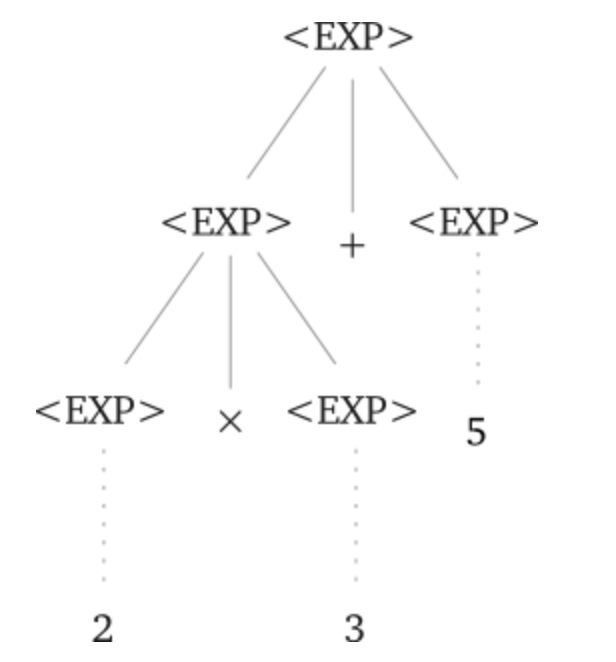
\includegraphics[scale = 0.6]{images/1}
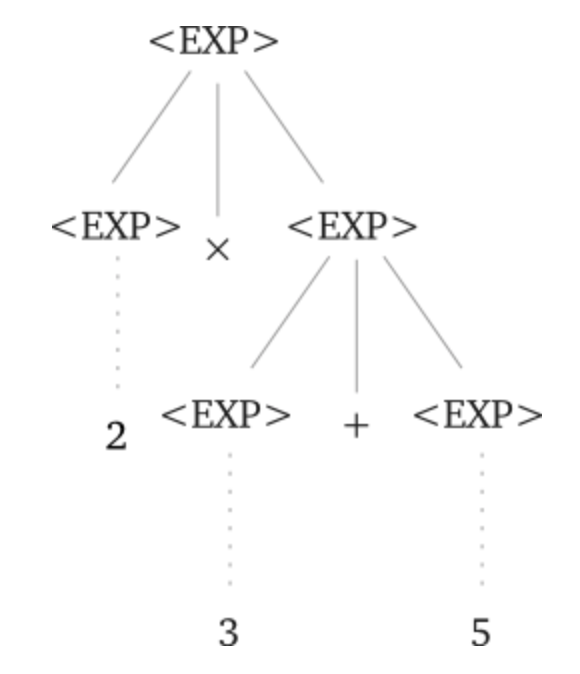
\includegraphics[scale = 0.6]{images/2}\\\\
\textbf{October 17th Lecture 15}\\
So, we need to build a new grammar:	
\begin{itemize}
	\item $V\text{ (non-terminals) } = \curbrak{\ \lrangle{EXP}, \lrangle{TERM}, \lrangle{FACTOR}\ }$
	\item Start Symbol $\lrangle{EXP}$
	\item $<EXP>\ \to\  <EXP>+<TERM>\ | \ <TERM>$
	\item $<TERM>\ \to \ <TERM>\times <FACTOR>\ |\ <FACTOR> $
	\item $<FACTOR>\ \to \ <NUM>\ |\ (<EXP>)$
\end{itemize}
Then, the only derivation tree for $2\times 3+5$ is the following:\\
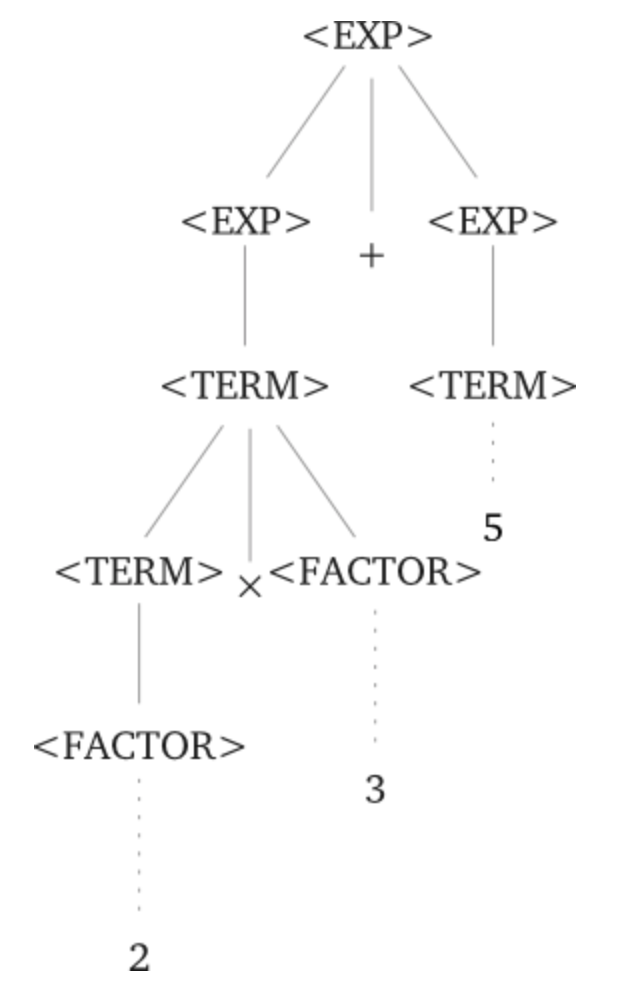
\includegraphics[scale = 0.5]{images/3}
\newpage
We couldn't generate a different tree for the expression if we tried - if we tried to group it the other way as we did above (by evaluating 3+5
first), then we would generate the expression $2\times (3+5)$, which is not the same string.\\
\\
\textbf{REMARK: } Tree structure is important for meaning.\\
\\
\textbf{EXAMPLE 1:}\\
$L = \curbrak{\ a^n b^{2n} \ |\ n \geq 0\ } \quad \quad S\to aSbb \ |\ \varepsilon$\\
\\
\textbf{EXAMPLE 2:}\\
$L = \curbrak{\ X \ |\ X = X^{rev}\ } \quad \quad \Sigma = \curbrak{\ a, b \ }\quad\quad  S\to aSa \ |\ bSb \ |\  \varepsilon \ |\ a \ |\ b $
\\
\\
\textbf{EXAMPLE 3:}\\
$L = \curbrak{\ X\in \Sigma^* \ |\ X \text{ has as many a's as b's }\ } \quad \quad \Sigma = \curbrak{\ a, b \ }$\\
We define a function $d(x) = \#b(x) - \#a(x)$, then $L = \curbrak{\ x\ |\ d(x) = 0\ }$\\
\\
Suppose that $u \in L$, then we can say $u$ has the same number of a's as the number of b's.\\
And we assume that $u$ starts with an $a$\quad \quad $u = aw\quad d(w) = 1$\\\\
Let $x$ be the \textbf{shortest} prefix such that $d(x) = 0$, then we know that the last letter of $x$ is $b$.\\
If the last letter of $x$ is $a$, then we know that it can't be the shortest prefix such that $d(x) = 0$, there must exist shorter prefix.\\
Suppose $u = xy$, since for x, we have $d(x) = 0$, we also have $d(y) = 0$\\\\
x must be in this form $x = aVb \quad$then we have $u = xy = aVby \quad V, y \in L$\\\\
Thus, we have:
$$A: \quad\quad S \to aSbS \ |\ bSaS \ |\ \varepsilon \ or$$
$$B: \quad\quad S \to aSb \ |\ bSa \ |\ SS\ |\  \varepsilon $$
\\\\
\begin{itemize}
	\item Every word generated is in $L$
	\item Every word in $L$ can be generated
\end{itemize}
\begin{mdframed}
For $B$:\\
Obviously, any word generated by $B$ has the same number of a's and b's\\
\\
Now, we need to show that any word with same number of a's and b's can be generated.\\
We prove by induction of the number of a's.\\\\
Base Case: $\varepsilon$, obviously, this is true.\\\\
Inductive Step: assume that the word contains $n$ a's and $n$ b's can be generated.\\	
Consider string with $(n+1)$ a's and  $(n+1)$ b's:\\
$$ awb \implies S\to aSb \quad\quad bwa \implies S\to bSa $$
Suppose that $w$ begins and ends with a\quad $w = a w' a$, which means $w'$ has 2 more b's than a's.\\
Thus, we can separate $w'$ as $w' = w'_1 w'_2$, where $w'_1$ has one more b than a so is $w'_2$.\\
Thus, we can write $w'$ as $w' = a w'_1 w'_2 a$\quad\quad where $aw_1'$ has same number of a and b so is $w_2'$\\
According to our hypothesis, we can rewrite $aw_1'$ according to rule $S \to aSb$
we can rewrite $w_2'a$ according to rule $S \to bSa$, 
which means $w$ can be rewritten as $w = SS$

\end{mdframed}

\textbf{FACT:} If you have a function behave like $d(x)$ defined before, which can only change by $\pm 1$ at each step, it starts at negative and ends up at positive, then it must hit 0.\\
\\
\\





\section*{Chomsky Normal Form:}
Every CFL has a grammar in which the rules are of a very restricted form, which is:	
\begin{itemize}
	\item $A \to a$
	\item $A \to BC$
\end{itemize}
Where $A, B, C$ are non-terminal.\\
Note that $A\to \varepsilon $ is not allowed except when $A=S$.\\
\\
\\
\textbf{October 19th Lecture 16}
\subsection*{Recognize a CFL}
\textbf{Push Down Automata \quad PDA \quad (stack machine) $\implies$  DFA + 1 stack} \\
Recall: $\{ a^n b^n\ |\ n \geq 0 \}$, which is non-regular\\
CFL recognized by PDA:\\
\begin{itemize}
	\item $Q$: states \quad $\Sigma$: alphabet(input) \quad $\Gamma$: stack alphabet 
	\item $q_0$: start state \quad $F \subseteq Q$ accept 
	\item $\Sigma_\varepsilon = \Sigma \cup \{ \varepsilon \}$ \quad $\Gamma_{\varepsilon} = \Gamma\cup \{ \varepsilon \}$
	\item $\delta: Q \times \Sigma_{\varepsilon} \times \Gamma_{\varepsilon} = \mathcal{P}_{finite}(Q \times \Gamma_{\varepsilon} )$ \quad \quad finite power set
\end{itemize}
Look at input and top of stack, then pop the stack, push a new symbol, change state.\\
\\
We decorate arrows with $a, b \to c$\\
See $a$ in the input, $b$ on the top of the stack $\implies$ replace $b$ with $c$ on the stack
$$ a = \varepsilon \quad \text{don't look at input} \quad \quad b = \varepsilon \quad \text{just push c}\quad \quad c = \varepsilon \quad \text{just pop b} $$
\newpage
$$ L = \{\ 0^n 1^n | n \geq 0\ \} $$
\begin{center}
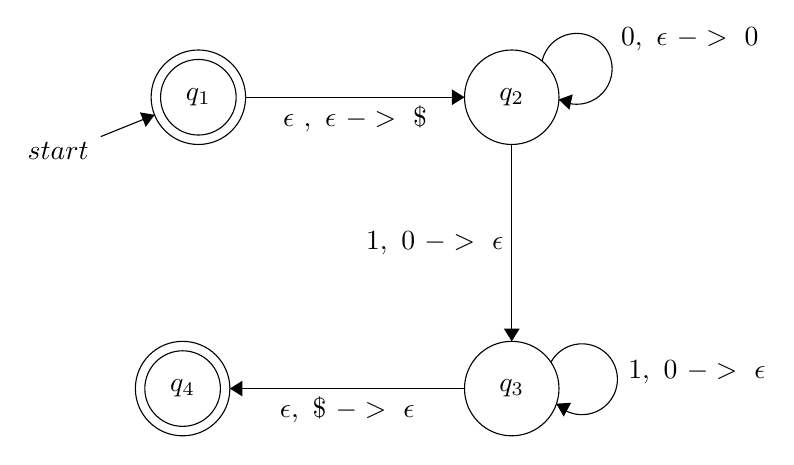
\begin{tikzpicture}[scale=0.2]
\tikzstyle{every node}+=[inner sep=0pt]
\draw [black] (15.7,-21.1) circle (3);
\draw (15.7,-21.1) node {$q_1$};
\draw [black] (15.7,-21.1) circle (2.4);
\draw [black] (35.6,-21.1) circle (3);
\draw (35.6,-21.1) node {$q_2$};
\draw [black] (35.6,-39.6) circle (3);
\draw (35.6,-39.6) node {$q_3$};
\draw [black] (14.7,-39.6) circle (3);
\draw (14.7,-39.6) node {$q_4$};
\draw [black] (14.7,-39.6) circle (2.4);
\draw [black] (9.5,-23.6) -- (12.92,-22.22);
\draw (8.76,-24.49) node [left] {$start$};
\fill [black] (12.92,-22.22) -- (11.99,-22.06) -- (12.36,-22.98);
\draw [black] (18.7,-21.1) -- (32.6,-21.1);
\fill [black] (32.6,-21.1) -- (31.8,-20.6) -- (31.8,-21.6);
\draw (25.65,-21.6) node [below] {$\epsilon\mbox{ },\mbox{ }\epsilon\mbox{ }->\mbox{ }\$ $};
\draw [black] (35.6,-24.1) -- (35.6,-36.6);
\fill [black] (35.6,-36.6) -- (36.1,-35.8) -- (35.1,-35.8);
\draw (35.1,-30.35) node [left] {$1,\mbox{ }0\mbox{ }->\mbox{ }\epsilon$};
\draw [black] (37.525,-18.814) arc (167.62938:-120.37062:2.25);
\draw (42.51,-17.42) node [right] {$0,\mbox{ }\epsilon\mbox{ }->\mbox{ }0$};
\fill [black] (38.59,-21.24) -- (39.26,-21.9) -- (39.47,-20.92);
\draw [black] (38.082,-37.936) arc (151.56226:-136.43774:2.25);
\draw (42.97,-38.56) node [right] {$1,\mbox{ }0\mbox{ }->\mbox{ }\epsilon$};
\fill [black] (38.43,-40.56) -- (38.9,-41.38) -- (39.37,-40.5);
\draw [black] (32.6,-39.6) -- (17.7,-39.6);
\fill [black] (17.7,-39.6) -- (18.5,-40.1) -- (18.5,-39.1);
\draw (25.15,-40.1) node [below] {$\epsilon,\mbox{ }\$ \mbox{ }->\mbox{ }\epsilon$};
\end{tikzpicture}
\end{center}
$$ \$ : \text{ special symbol to indicate the end of stack }$$
\\
\\
$$ L = \{\ a^i b^j c^k \ |\ i, j, k \geq 0 \quad i = j \ or\  i = k \ \} $$
\begin{center}
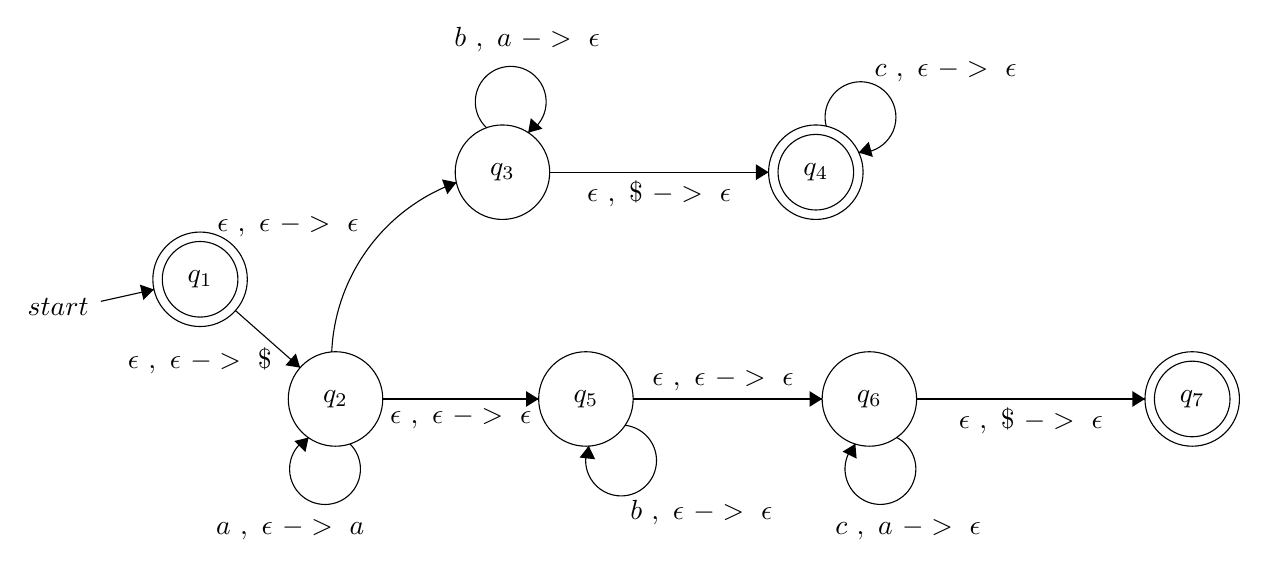
\begin{tikzpicture}[scale=0.2]
\tikzstyle{every node}+=[inner sep=0pt]
\draw [black] (12,-23.8) circle (3);
\draw (12,-23.8) node {$q_1$};
\draw [black] (12,-23.8) circle (2.4);
\draw [black] (20.6,-31.4) circle (3);
\draw (20.6,-31.4) node {$q_2$};
\draw [black] (31.2,-17) circle (3);
\draw (31.2,-17) node {$q_3$};
\draw [black] (36.5,-31.4) circle (3);
\draw (36.5,-31.4) node {$q_5$};
\draw [black] (54.5,-31.4) circle (3);
\draw (54.5,-31.4) node {$q_6$};
\draw [black] (75,-31.4) circle (3);
\draw (75,-31.4) node {$q_7$};
\draw [black] (75,-31.4) circle (2.4);
\draw [black] (51.1,-17) circle (3);
\draw (51.1,-17) node {$q_4$};
\draw [black] (51.1,-17) circle (2.4);
\draw [black] (5.7,-25.2) -- (9.07,-24.45);
\draw (4.95,-25.58) node [left] {$start$};
\fill [black] (9.07,-24.45) -- (8.18,-24.14) -- (8.4,-25.11);
\draw [black] (14.25,-25.79) -- (18.35,-29.41);
\fill [black] (18.35,-29.41) -- (18.08,-28.51) -- (17.42,-29.26);
\draw (11.98,-28.09) node [below] {$\epsilon\mbox{ },\mbox{ }\epsilon\mbox{ }->\mbox{ }\$ $};
\draw [black] (21.51,-34.246) arc (45.46923:-242.53077:2.25);
\draw (18.02,-38.97) node [below] {$a\mbox{ },\mbox{ }\epsilon\mbox{ }->\mbox{ }a\mbox{ }$};
\fill [black] (18.89,-33.85) -- (17.98,-34.07) -- (18.69,-34.77);
\draw [black] (20.358,-28.418) arc (-182.51416:-250.20023:11.999);
\fill [black] (28.28,-17.65) -- (27.36,-17.46) -- (27.7,-18.4);
\draw (22.1,-20.44) node [left] {$\epsilon\mbox{ },\mbox{ }\epsilon\mbox{ }->\mbox{ }\epsilon$};
\draw [black] (30.2,-14.184) arc (227.29016:-60.70984:2.25);
\draw (33.06,-9.42) node [above] {$b\mbox{ },\mbox{ }a\mbox{ }->\mbox{ }\epsilon\mbox{ }$};
\fill [black] (32.83,-14.49) -- (33.74,-14.24) -- (33,-13.57);
\draw [black] (38.978,-33.07) arc (83.74488:-204.25512:2.25);
\draw (44.12,-37.77) node [below] {$b\mbox{ },\mbox{ }\epsilon\mbox{ }->\mbox{ }\epsilon\mbox{ }$};
\fill [black] (36.68,-34.38) -- (36.1,-35.12) -- (37.09,-35.23);
\draw [black] (23.6,-31.4) -- (33.5,-31.4);
\fill [black] (33.5,-31.4) -- (32.7,-30.9) -- (32.7,-31.9);
\draw (28.55,-31.9) node [below] {$\epsilon\mbox{ },\mbox{ }\epsilon\mbox{ }->\mbox{ }\epsilon$};
\draw [black] (39.5,-31.4) -- (51.5,-31.4);
\fill [black] (51.5,-31.4) -- (50.7,-30.9) -- (50.7,-31.9);
\draw (45.5,-30.9) node [above] {$\epsilon\mbox{ },\mbox{ }\epsilon\mbox{ }->\mbox{ }\epsilon\mbox{ }$};
\draw [black] (56.224,-33.841) arc (62.97263:-225.02737:2.25);
\draw (57.26,-38.97) node [below] {$c\mbox{ },\mbox{ }a\mbox{ }->\mbox{ }\epsilon\mbox{ }$};
\fill [black] (53.61,-34.25) -- (52.8,-34.74) -- (53.69,-35.19);
\draw [black] (57.5,-31.4) -- (72,-31.4);
\fill [black] (72,-31.4) -- (71.2,-30.9) -- (71.2,-31.9);
\draw (64.75,-31.9) node [below] {$\epsilon\mbox{ },\mbox{ }\$ \mbox{ }->\mbox{ }\epsilon$};
\draw [black] (51.763,-14.086) arc (194.90614:-93.09386:2.25);
\draw (59.34,-11.27) node [above] {$c\mbox{ },\mbox{ }\epsilon\mbox{ }->\mbox{ }\epsilon$};
\fill [black] (53.82,-15.75) -- (54.72,-16.03) -- (54.46,-15.07);
\draw [black] (34.2,-17) -- (48.1,-17);
\fill [black] (48.1,-17) -- (47.3,-16.5) -- (47.3,-17.5);
\draw (41.15,-17.5) node [below] {$\epsilon\mbox{ },\mbox{ }\$ \mbox{ }->\mbox{ }\epsilon$};
\end{tikzpicture}
\end{center}

\textbf{Theorem:}
\begin{itemize}
	\item Every CFL is recognized by some PDA
	\item Every language recognized by a PDA is a CFL
	\item the intersection of a CFL and a regular language  = CFL
	\item the intersection of 2 CFL MAY NOT BE a context free.
\end{itemize}


\end{document}